\documentclass{article}
\usepackage{graphicx}
\begin{document}
	\section{MOBILE PHONES}
	A mobile phone (or cellphone[a]) is a portable telephone that can make and receive calls over a radio frequency link while the user is moving within a telephone service area, as opposed to a fixed-location phone (landline phone). The radio frequency link establishes a connection to the switching systems of a mobile phone operator, which provides access to the public switched telephone network (PSTN). Modern mobile telephone services use a cellular network architecture, and therefore mobile telephones are called cellphones (or "cell phones") in North America. In addition to telephony, digital mobile phones support a variety of other services, such as text messaging, multimedia messaging, email, Internet access (via LTE, 5G NR or Wi-Fi), short-range wireless communications (infrared, Bluetooth), satellite access (navigation, messaging connectivity), business applications, payments (via NFC), multimedia playback and streaming (radio, television), digital photography, and video games. Mobile phones offering only basic capabilities are known as feature phones (slang: "dumbphones"); mobile phones that offer greatly advanced computing capabilities are referred to as smartphones.[1]
	
	
\begin{figure}
	\centering
	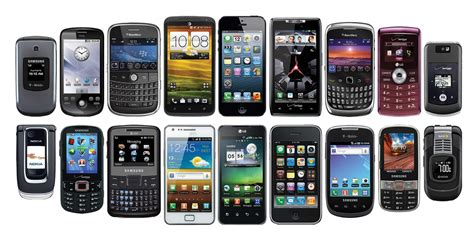
\includegraphics[width=0.7\textwidth]{m.jpg}
	\caption{ mobiles}
	\label{fig:mobile phones}
\end{figure}

	The first handheld mobile phone was demonstrated by Martin Cooper of Motorola in New York City on 3 April 1973, using a handset weighing c. 2 kilograms (4.4 lbs).[2] In 1979, Nippon Telegraph and Telephone (NTT) launched the world's first cellular network in Japan.[3] In 1983, the DynaTAC 8000x was the first commercially available handheld mobile phone. From 1983 to 2014, worldwide mobile phone subscriptions grew to over seven billion; enough to provide one for every person on Earth.[4] In the first quarter of 2016, the top smartphone developers worldwide were Samsung, Apple and Huawei; smartphone sales represented 78 percent of total mobile phone sales.[5] For feature phones as of 2016, the top-selling brands were Samsung, Nokia and Alcatel.[6]

	Mobile phones are considered an important human invention as they have been one of the most widely used and sold pieces of consumer technology.[7] The growth in popularity has been rapid in some places, for example, in the UK, the total number of mobile phones overtook the number of houses in 1999.[8] Today, mobile phones are globally ubiquitous,[9] and in almost half the world's countries, over 90% of the population owns at least one.[10]

\end{document}